\subsection{Market Making}
O market-making é uma forma de negociação (\textit{trading} em inglês) que de forma simplificada consiste em comprar certo ativo a um determinado preço e vender-lo a um preço maior.
Como os preços de compra e venda dos ativos são afetados pela demanda e oferta no momento, cada agente no mercado exerce certa influência sobre o valor de um ativo, a depender das ofertas que o mesmo mantém para tal ativo no livro de ordens limite (\textit{limit order book}, ou \textit{LOB} em inglês). 

No \textit{LOB} os registros se dão primeiramente por ordem de preço, e em segundo por data de criação: as ofertas com melhor preço (tanto para compra como para venda) ficam no topo do livro, e caso tenham o mesmo valor entre si tem sua posição desempatada pela ordem temporal de chegada. No livro de compras, a melhor oferta é a que oferece o maior preço, e o contrário vale para o livro de vendas.

Nas bolsas de valores digitais a execução de uma transação é automática e auxiliada por um sistema chamado de \textit{matching engine} - ou seja, um motor para pareamento de ordens. Esse sistema verifica se para a melhor oferta de compra (ou venda) existe outra correspondente no livro de venda (ou compra) com valor menor ou igual (ou maior ou igual para venda). Após o pareamento, a bolsa anuncia o a execução da ordem e as ofertas relacionadas são removidas dos livros.

Em suma, os principais elementos do market making incluem, mas não se limitam à:

\begin{itemize}
	\item Spread: É a diferença entre o preço de compra (\textit{bid} em inglês) e o preço de venda (\textit{ask} em inglês) entre duas ofertas. O market maker busca obter os melhores valores para esses preços, e eventualmente lucrar com a diferença entre eles.
	
	\item Livro de Ordens Limite: É um conjunto ordenado onde as ofertas de compra e venda são registradas. Também é permitido o ajuste dos preços de compra e venda de ofertas existentes por parte dos agentes.
	
	\item Gestão de Risco: Todos \textit{market-makers} enfrentam riscos em suas negociações, entre eles o risco de inventário e risco de mercado. O risco de inventário ocorre quando o market maker mantém uma posição desequilibrada entre ativos comprados e vendidos, enquanto o risco de mercado está relacionado às flutuações nos preços dos ativos.
\end{itemize}

No contexto deste projeto, o foco da pesquisa será a otimização de uma estratégia de \textit{market-making} que minimize o risco de inventário durante a noite. A estratégia será composta por um agente responsável pela interação com o mercado e alocação de preços sob políticas para redução de risco. Mais adiante, será apresentado a modelagem do problema como uma cadeia de decisão de Markov. Tendo definido o espaço de ações possíveis para o agente e de observações possíveis do mercado, modelaremos a equação de otimalidade de Bellman para os estados do mercado, e discutiremos os algoritmos de Aprendizado por Reforço (RL) que foram escolhidos como abordagem para obter um agente ótimo capaz de aproximar numericamente os preços ótimos.

\subsection{Sistemas dinâmicos e Aprendizado por Reforço}
O Aprendizado por Reforço (RL) é um paradigma de aprendizado baseado em princípios da psicologia comportamental e em otimização estocástica, especificamente tarefas de controle e sistemas dinâmicos. Simplificadamente, trata-se de uma técnica para modelagem, simulação e treino de um agente. Tal agente é capaz de interagir com um ambiente, modelado a partir de um processo de decisão de Markov, com o objetivo de obter uma política de interação com o sistema que maximize sua recompensa cumulativa ao longo do tempo, chamada de "retorno" (note que no contexto de \textit{RL}, o retorno é diferente do retorno financeiro em si).

\begin{figure}[H]
	\centering
	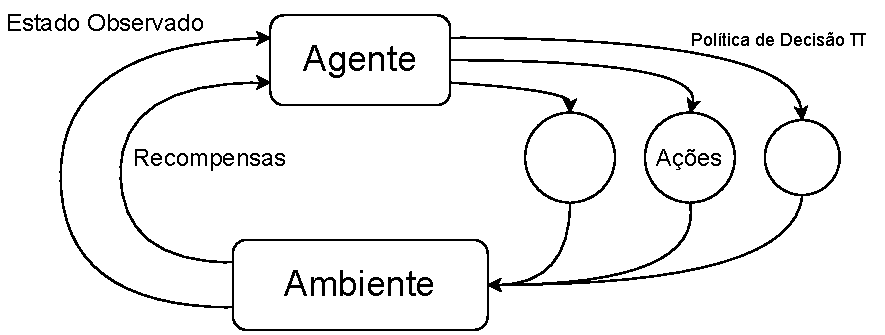
\includegraphics{files/rl-agent.pdf}
	\caption{Autômato do Agente sob o paradigma de Aprendizado por Reforço}
	\label{fig:rl-agent}
\end{figure}

A definição de uma cadeia de decisão com a qual o agente interagirá é uma tupla $MDP = (\mathcal{S}, \mathcal{A}, T_{a}, R_{a})$, onde os elementos que a compõem são:

\begin{description}
	\item[$\mathcal{S}$] 
	é o espaço de estados possíveis, representado por um conjunto de estados, onde cada estado $s \in \mathcal{S}$ é uma tupla de $n$ valores numéricos observáveis $s = (x_{0}, x_{1}, \ldots, x_{n})$. Cada estado é uma observação possível da dinâmica do sistema em determinado momento;
	
	\item[$\mathcal{A}$] é o espaço de ações que o agente pode realizar. Uma ação $a \in \mathcal{A}$ é uma tupla com $m$ valores numéricos tal que $a = (y_{0}, y_{1}, \ldots, y_{m})$ são os valores que o agente aplica no sistema, e transiciona à um novo estado, recebendo uma recompensa.
	
	\item[\textit{T}] é o operador de transição, que representa as transições possíveis entre estado atual $s$ e possível estado futuro $s'$, dado uma ação $a$ tomada pelo agente, tal qual \(T : \mathcal{S} \times \mathcal{A} \times \mathcal{S} \rightarrow [0, 1]\). A função $T$ fornece uma função de densidade de probabilidade, tal que $T(s, a, s') = f(s' \,|\, s, a)$ onde \(f(s' \,|\, s, a) \in \mathcal{L}([0, 1])\) e $\mathcal{L}$ é o espaço de probabilidade padrão de Lebesgue.
	
	\item[\textit{R}] é a função de recompensa da cadeia de markov, que mapeia uma determinada transição à probabilidade de uma recompensa ocorrer 
	$R : \mathcal{S} \times \mathcal{A} \times \mathcal{S} \rightarrow \mathbb{R}$, onde $R(s, a, s') = \int_{\mathbb{R}} r \cdot f(r \,|\, s, a, s') \, dr$ e $f$ é a função de densidade condicional à transição ocorrida, e a integral retorna o valor esperado da recompensa.
\end{description}

\begin{figure}[H]
	\centering
	\documentclass[tikz,border=10pt]{standalone}
\usepackage{pgf}
\usepackage{xcolor}

\begin{document}
	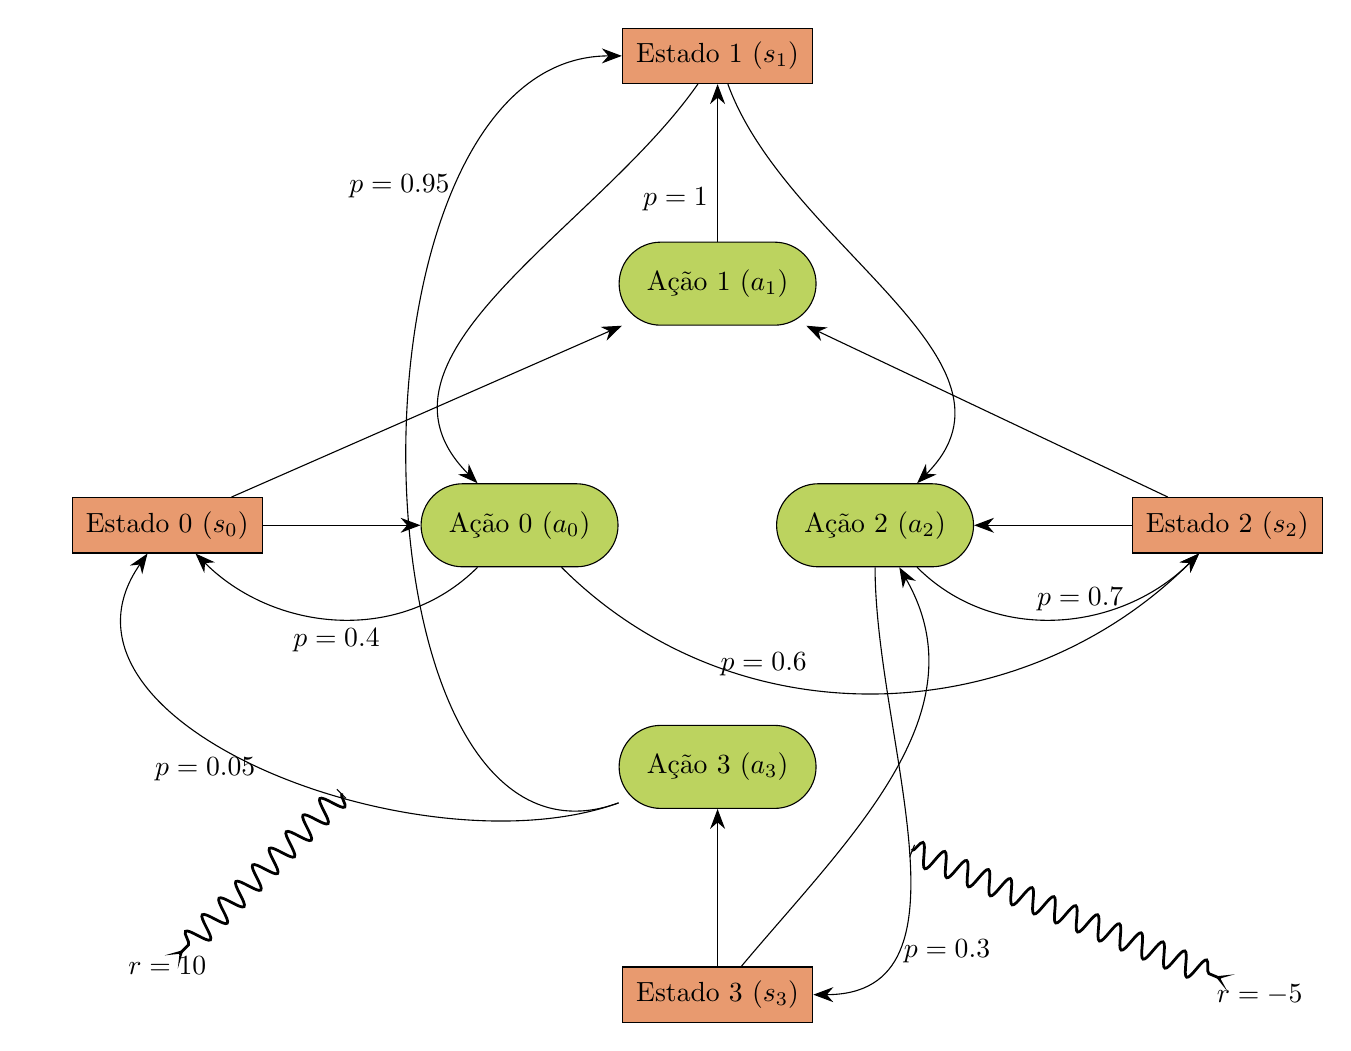
\begin{tikzpicture}
		\usetikzlibrary{arrows,automata,positioning,arrows.meta};
		\definecolor{statecolor}{HTML}{e89a6f};
		\definecolor{actioncolor}{HTML}{bcd35f};
		\tikzset{
			state/.style={
				shape=rectangle,
				draw=black,
				fill=statecolor,
				align=center,
				minimum height=2em,
				minimum width=4em,
				inner sep=5pt,
			},
			action/.style={
				shape=rectangle,
				draw=black,
				fill=actioncolor,
				align=center,
				inner sep=10pt,
				rounded corners=15pt,
			},
			reward/.style={
				|-,
				decoration={snake, amplitude=1.5mm, segment length=3mm},
				decorate,
				postaction={draw, line width=1pt, -{Stealth[scale=-0.8]}}
			},
			transition/.style={
				->,
				>={Stealth[scale=1.5]},
			}
		};
		\tikzset{node distance=2cm and 2cm}
    	\node[state] (s0) {Estado 0 ($s_0$)};

		\node[action, right=2cm of s0] (a0) {Ação 0 ($a_0$)};
		\node[action, above right=2cm and 0cm of a0] (a1) {Ação 1 ($a_1$)};
		\node[action, right=2cm of a0] (a2) {Ação 2 ($a_2$)};
		\node[action, below right=2cm and 0cm of a0] (a3) {Ação 3 ($a_3$)};

		\node[state, above=2cm of a1] (s1) {Estado 1 ($s_1$)};
		\node[state, right=2cm of a2] (s2) {Estado 2 ($s_2$)};
		\node[state, below=2cm of a3] (s3) {Estado 3 ($s_3$)};
		
		\node[draw=none, below right=2.8cm and 1cm of s0] (r0s) {};
		\node[draw=none, below=5cm of s0] (r0e) {$r=10$};
		
		\node[draw=none, above right=1.4cm and 1cm of s3] (r1s) {};
		\node[draw=none, right=5cm of s3] (r1e) {$r=-5$};
		
		\begin{scope} % actions
			\draw[transition] 
			(s0) 
			to
			(a0);
	
			\draw[transition] 
			(s0) 
			to
			(a1);
	
			\draw[transition] 
			(s1) 
			to[in=45, out=290]
			(a2);
	
			\draw[transition] 
			(s1) 
			to[in=135, out=235]
			(a0);
	
			\draw[transition] 
			(s2) 
			to
			(a1);
	
			\draw[transition] 
			(s2) 
			to
			(a2);
	
			\draw[transition] 
			(s3) 
			to
			(a3);
	
			\draw[transition] 
			(s3) 
			to[in=300, out=50]
			(a2);		
		\end{scope}
		
		\begin{scope} % transitions
			\draw[transition] 
			(a0)
			to[in=315, out=225] node[midway, below] 
			{$p = 0.4$} 
			(s0);
			
			\draw[transition] 
			(a0) 
			to[in=225, out=315] node[near start, right] 
			{$p = 0.6$} 
			(s2);
			
			\draw[transition] 
			(a1) 
			to[in=270, out=90] node[near start, left] 
			{$p = 1$} 
			(s1);
			
			\draw[transition] 
			(a2) 
			to[in=225, out=315] node[near end, left] 
			{$p = 0.7$} 
			(s2);
			
			\draw[transition] 
			(a2) 
			to[in=0, out=270] node[near end, right] 
			{$p = 0.3$} 
			(s3);
			
			\draw[transition] 
			(a3) 
			to[in=235, out=200] node[midway, left] 
			{$p = 0.05$} 
			(s0);
			
			\draw[transition] 
			(a3) 
			to[in=180, out=200] node[near end, left] 
			{$p = 0.95$} 
			(s1);
		\end{scope}
		
		\begin{scope}
			\draw[reward]
			(r0s)
			to
			(r0e);
			
			\draw[reward]
			(r1s)
			to
			(r1e);
			
		\end{scope}
	\end{tikzpicture}
\end{document}

	\caption{Processo de Decisão de Markov com 4 estados e 4 ações (MDP)}
	\label{fig:mdp}
\end{figure}

Considerando o contexto de controle estocástico, um agente ou controle é efetivamente a política de escolha de ações. Dado um estado atual $s$ e uma ação $a$, a política dá a probabilidade do agente executar e enviar à cadeia tal ação. Uma política estocástica $\pi$ qualquer é representada por:

\begin{equation}
	\begin{aligned}
	\pi(a \,|\, s) = g(a \,|\, s)\text{, onde }\\ g(a \,|\, s) \in \mathcal{L}([0, 1])
	\end{aligned}
\end{equation}

Por fim, o objetivo do agente é obter uma política ótima que maximize o retorno obtido, que é a soma amortizada das recompensas futuras. O retorno do agente é obtida pela seguinte expressão, para um determinado momento em um intervalo de tempo discreto $t \leq T, t \in \mathbb{Z}$, onde T é o final do período de observação:

\begin{equation}
	\begin{aligned}
		G_{t} = \sum_{k=0}^{T} \gamma^t \cdot R_{t + k + 1}
	\end{aligned}
\end{equation}

onde $\gamma$ é o fator de amortecimento e $R_t$ é a recompensa que o agente recebe no momento $t$, de acordo com uma função de recompensa $R$, ou seja $R_t = R(s_{t}, a_{t}, s_{t + 1})$.

De modo a obter a política que maximize o retorno do agente, é necessário definir duas equações importantes para o contexto de aprendizado por reforço. A função de valor de estado de Bellman \(V_\pi(s)\) quantifica o retorno cumulativo esperado quando um agente começa no estado \(s\) e segue uma política específica \(\pi\):
\[ 
V^{\pi}(s) = \mathbb{E}_\pi[G_t | S_t = s]
\]
onde \(G_t\) é o retorno no tempo e \(S_t\) é o estado no tempo \(t\).

A função de valor de estado-ação, \(Q_\pi(s, a)\), estende a função de valor do estado ao considerar tanto o estado atual \(s\) quanto uma ação escolhida \(a\):
\[ Q^{\pi}(s, a) = \mathbb{E}_\pi[G_t | S_t = s, A_t = a]\]
onde \(A_t\) é a ação tomada no tempo \(t\).

A equação estado-valor de otimalidade, \(V^*(s)\), representa o retorno cumulativo máximo esperado alcançável a partir do estado \(s\) entre todas as políticas possíveis:
\[ V^*(s) = \max_\pi V^{\pi}(s). \]

Por fim, a política ótima $\pi^*$ é obtida ao selecionar ações que maximizam a função de valor de estado-ação:
\[ \pi^*(a|s) = \arg\max_a Q^*(s, a), \]
onde \(Q^*(s, a)\) é a função de valor de estado-ação ótima.

Os valores de $Q^{*}$ não são conhecidos para sistemas mais complexos, assim como não são discretizáveis para problemas com espaços de ação ou estado contínuos. Na próxima seção será discutido as técnicas e metodologias possíveis para se obter os valores da equação de estado ação de otimalidade, assim como a necessidade do uso do aprendizado por reforço devido à complexidade de ambientes como bolsas digitais e livros de ordem limite.
